% Explain how the CLI is implemented.
The \emph{CLI} is very simple and works by having a thread that constantly waits for an input from the command line.
When an input is given to the thread it tries to parses the input into a request for the debugger.
It parses the input by first comparing the fist word of the input to all the commands, if it matches a command then the rest of the input is parsed by using the specific parser for that command.
If the input does not mach any of the commands then an error is printed to the user.
When the input has been parsed into a request it is then sent through a channel to the main thread which forwards it to the debug thread.
Then when the main thread gets a response back from the debug thread it prints the result to the user and sends a boolean back to the thread that reads the input.
The boolean tells the thread if it should continue reading inputs or if it should stop.
The main tread constantly awaits a request form the input thread or a response or event from the debug thread.
It does this by constantly polling the two channels.
If the main thread receives a event from the debug event is displays it to the user and continues as usual.


\begin{figure}[h]
    \centering
    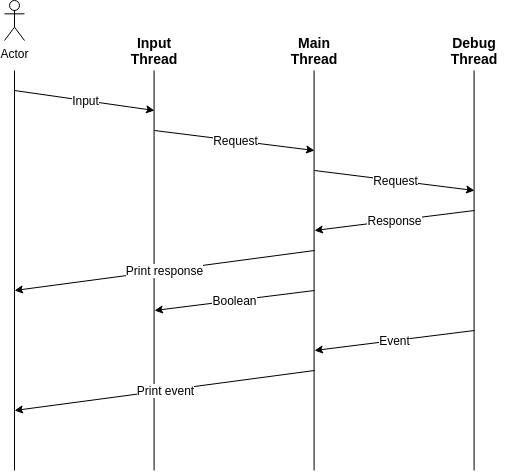
\includegraphics[width=1.0\textwidth]{cli_flow.png}
    \label{fig:cliflow}
\end{figure}

